The STK1000 provides a general purpose input/output interface (\texttt{GPIO}) with 32 signal lines.
16 of the 32 available lines were connected to on-board I/O devices on the STK1000 in this assignment.
The I/O devices in use were 8 on-board LEDs, used as a rudimentary paddle display, and 8 on-board switches, used as player controls.

The buttons were connected to \texttt{GPIO0-GPIO7} (\texttt{J1} on the STK1000) using a flat cable as in figure \ref{flat-cable-image}. This maps the buttons to ports \texttt{0-7} of \texttt{PIOB}.
The choice of low port numbers \texttt{0-7} is convenient for coding, and the choice of \texttt{PIOB} as opposed to \texttt{PIOC} is purely mnemonic ('B' for buttons).

The LEDs were connected to \texttt{GPIO16-GPIO23} (\texttt{J3} on the STK1000) using a flat cable as in figure \ref{flat-cable-image}. This maps the LEDs to ports \texttt{0-7} of \texttt{PIOC}.
Having the same port numbers for the buttons and the LEDs is a nice convenience for cleaner and more efficient code, as translation from button ports to LED ports is not necessary.

\begin{figure}
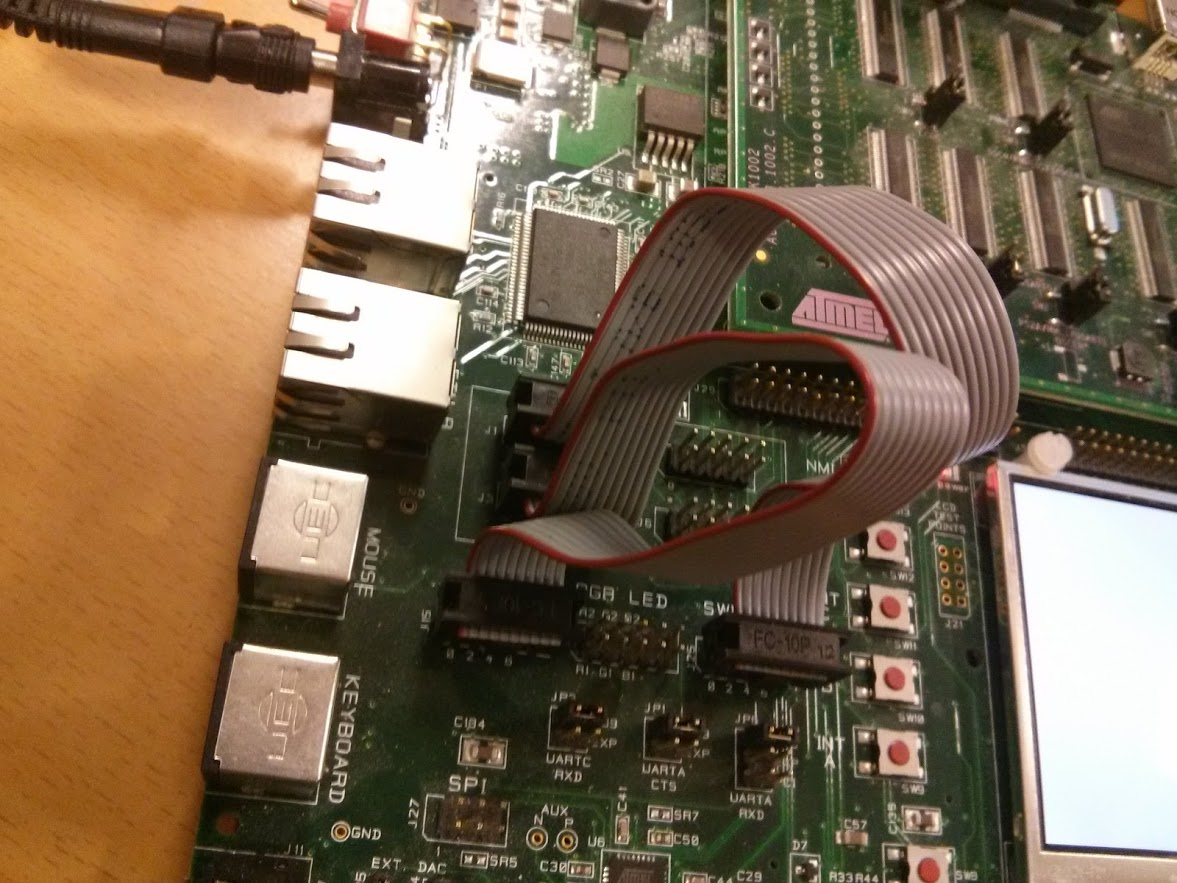
\includegraphics[width = \textwidth]{description-and-methodology/flat-cable-image.jpg}
\caption{Flat cables connecting \texttt{GPIO} with switches and LEDs. Note the orientation of the flat cables.}
\label{flat-cable-image}
\end{figure}
